\section{緒言}

\subsection{研究背景}

一般的に,流体はせん断応力がせん断速度に比例するNewton流体と,せん断応力がせん断速度が非線形となる非Newton流体に分類することができる.

Fig.\ref{fig:1-fluid-curve}(a)に示す通り,Newton流体はせん断速度とせん断応力が比例関係にある流体である.一方でそれ以外の流体は非Newton流体と呼ばれている.非Newton流体はDilatant fluid, Pseudoplastic, Bingham plastic, Viscoplastic, Viscoelastic が挙げられている.
非Newton流体のうち,Bingham plastic 流体, Viscoplastic 流体はせん断応力がある一定になるまでせん断速度が発生しない流体である.一方で,Dilatant fluid 流体, Pseudoplastic 流体はせん断応力が少しでも加わると,せん断速度が発生し流体的挙動を示す.また,Viscoelastic 流体は粘性だけでなく弾性的挙動を示す流体である.これら非Newton流体の粘度を示す理論として,Power-law model (Ostwald-De Waele model), Cross model,Carreau model,Carreau-Yasuda modelやHerschel-Bulkley modelなどを挙げることができる\cite{ref:1}.Power-law model はせん断速度の限られた範囲内にて適応することができる.理論式中の指数によってNewton流体,shear-thinning流体と,shear-thickening流体に分類することができる.これらのせん断速度と粘度の関係性はFig.\ref{fig:1-fluid-curve}(b)に示す通りである.これら2種類の流体のうち,本研究で扱うshear-thinning流体は,せん断速度$\dot{\gamma}$が高くなるほど粘度$\mu$が低くなる性質を有している.この流体は擬塑性流体とも呼ばれている.擬塑性流体の代表例として,泥や血液,ポリマーなどが挙げられる.本研究において試験溶液としたポリマーの流動は,粘性だけでなく弾性にも依存する\cite{viscoelasticity}.産業分野において,擬塑性流体の輸送を行うことがある.効率よく輸送を行うためには,せん断速度が高くなるほど粘度が低くなる性質を活かし,抵抗低減を図る必要がある.

Cross modelはshear-thinning性が構造的に引き起こされるといった仮説において導き出された理論である.これは広いせん断速度において適用することができる.また,Carreau model はCross modelをPower-law領域においてより適合するよう修正したものとなっている.Carreau-Yasuda model は,Carreau model を粘度減少が開始する特性時間に関してより適合するように修正されたものである.Herschel-Bulkley modelはBingham plasticやViscoplasticといった静止状態の流体においてせん断応力が存在する流体を示す理論となっている\cite{ref:1}.

流体中を運動する気泡や剛対に対する周囲流体の粘度分布,流動構造からその影響を明らかにする必要があり,様々な研究が行われてきた.例えば,Ohta {\it et al.} \cite{ref:2}は非弾性擬塑性流体中における液滴の上昇運動に対し,液滴周りのせん断速度による粘度低下があたえる影響を明らかにした.加えて,Ohta {\it et al.} \cite{ref:3}は液滴周りの粘度分布を数値計算より求め,局所的な粘度低下は液滴の形状に大きく依存することを明らかにした.また,Zhang {\it et al.} \cite{ref:4}は非弾性擬塑性流体中における単一気泡の上昇運動に対し,後方に生じる2つの高粘度領域が影響を与えることを明らかにした.

超音波振動の影響による抵抗低下に関してvan den Wildenberg {\it et al.}\cite{ref:6}による研究があげられる.本研究では,粒子の上部を水で満たした容器ごと振動させ,その粒子中に球を落下させた.その結果をFig.\ref{fig:4-sinking}に示す.Fig.\ref{fig:4-sinking}(a1)において,$\Gamma$は振動強度である.振動によって落下球表面におけるせん断応力が減少し,振動強度を強くするとより深くまで沈降すると報告された.Iwata {\it et al.}\cite{ref:5}は,擬塑性流体中における気泡の体積を超音波振動によって周期的に増加・減少させた.そのことにより,気泡周囲のせん断粘度が低下し,上昇速度が増加することを明らかにした.

また,Iwamuro \textit{et al}.\cite{ref:8}は擬塑性流体中を落下する球に超音波振動を照射し,流体物性,物体形状,超音波強度および周波数を変化させることで調査を行った.この場合,落下速度の高速化は音響境界層内部における粘度低下と,音響境界層の形成が関係していると明らかにした.しかし,調査された流体物性は限定的であり,粘性だけでなく弾性を有する試験流体おいて,弾性により高速化が抑制されることを示唆していた.
\begin{figure}[ht]
    \centering
    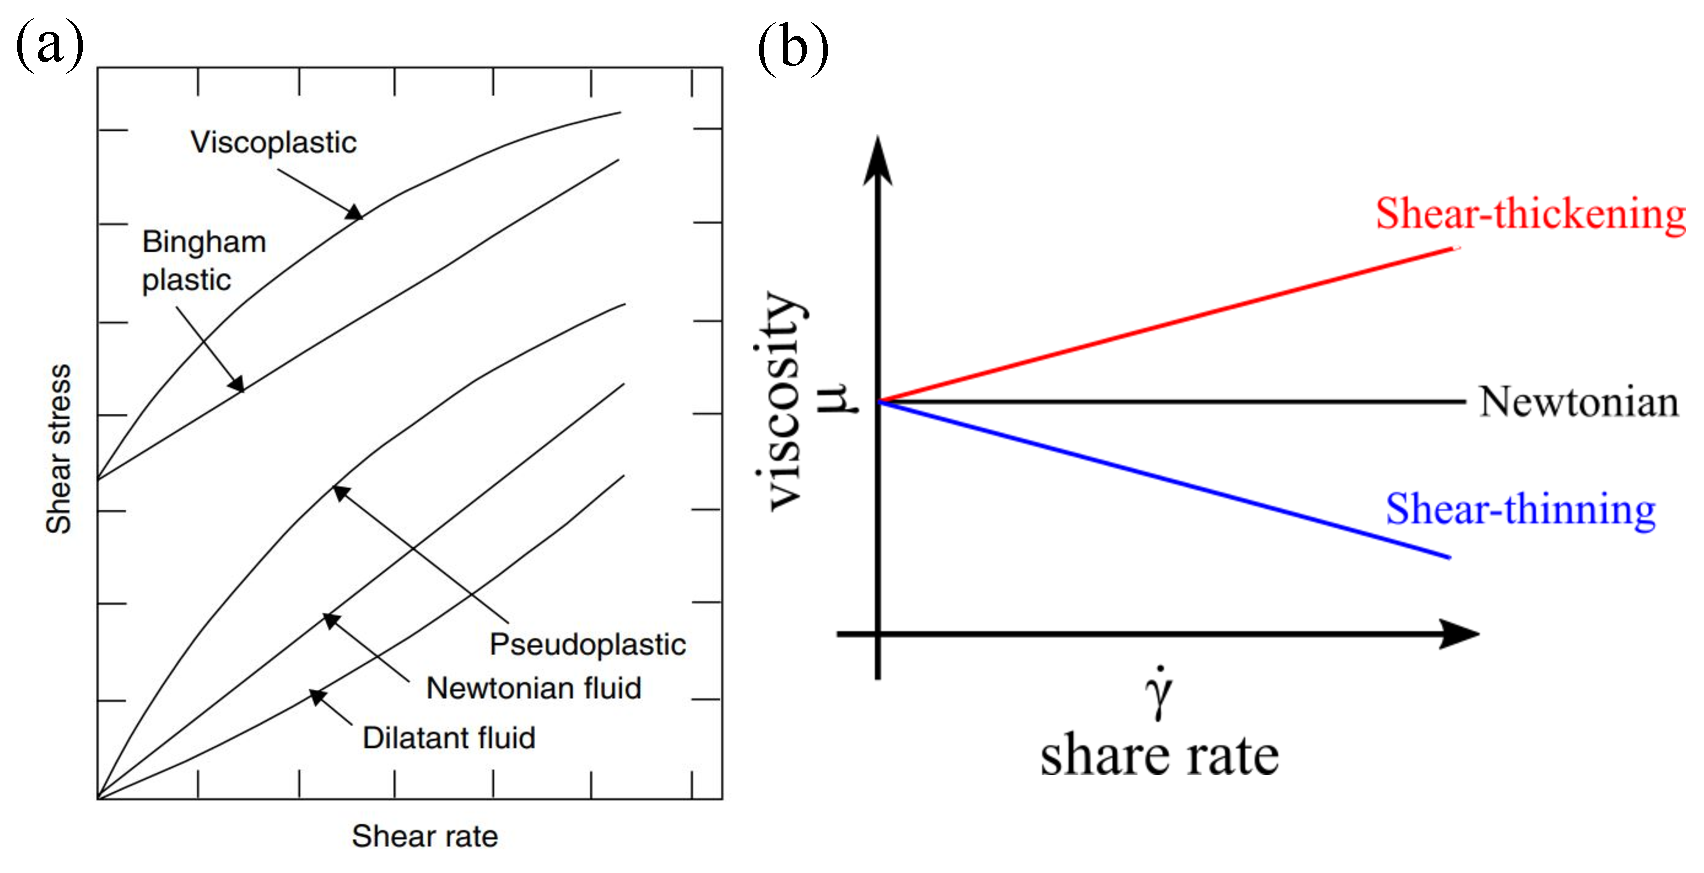
\includegraphics[width=1\textwidth]{1-Background/shea-thining.eps}
    \caption{(a) Qualitative flow curves for different types of non-Newtonian fluids\cite{ref:1}. (b)Classifications of non-Newtonian power-law fluid.}
    \label{fig:1-fluid-curve}
\end{figure}
\begin{figure}[ht]
    \begin{center}
        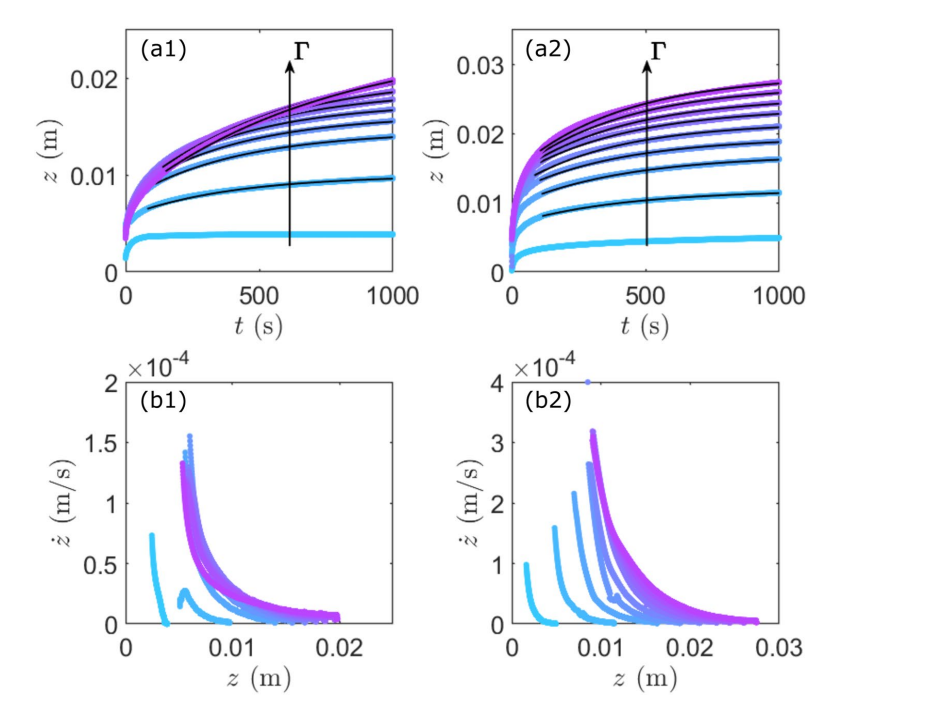
\includegraphics[width=11.0cm,clip]{1-Background/4-sinking.png}
        \caption{Sinking dynamics for different intruder-sizes and for different vibration intensities $\Gamma$. (a1) Depth versus time for an intruder with R=4mm and (a2) for an intruder with R=7mm. (b1) Instantaneous velocity versus sinking depth obtained from (a1) and (b2) from (a2). The black lines correspond to the solutions fitted in the quasi-steady regime\cite{ref:6}.}
        \label{fig:4-sinking}
    \end{center}
\end{figure}
\newpage
\subsection{研究目的}

先行研究\cite{ref:8}において,超音波照射された擬塑性流体中を落下する球の高速化の要因として,音響境界層内部における粘度低下と,音響境界層の形成が関係していると明らかにした.また,高速化が弾性によって抑制されることを示唆していた.しかし,調査された流体や落下球の種類,径は限定的であり,弾性が高速化抑制することを明らかにしていない.

本研究で用いた試験溶液では,球の落下による運動が高速の場合,粘性による影響が支配的であり,低速の場合は弾性による影響が支配的となる.落下球の終端速度を変化させることで粘性が支配的な場合と弾性が支配的な場合に分けて,超音波照射による高速化への影響を調査した.そこで,流体物性,落下物体の密度,落下球の径をより大きく変化させ実験を行った.超音波照射された擬塑性流体中を落下する球の高速化に対する粘弾性両方の影響を明らかにすることを目的とする.
